\chapter{Open Source Electric Power Engineering Software}
\label{sec:oss}
For the purposes of this thesis the Matlab source code from \matpower was
translated into the Python programming language and released as a project named
Pylon\footnote{http://packages.python.org/Pylon/} \cite{lincoln:pyreto}. It was
translated to allow existing implementations of policy gradient reinforcement
learning methods, from the PyBrain machine learning library \cite{schaul:2010},
to be coupled with \textsc{Matpower}'s scalable and extensible optimal power
flow formulations. With permission from the \matpower developers, the resulting
code was released under the terms of the Apache License, version~2.0, and this
section describes the project in the context of other open source Electrical
Power Engineering software tools to illustrate the contribution made.

%\begin{landscape}
%\begin{table}
\begin{sidewaystable}
%\vspace{1ex}
%\begin{small}
\begin{center}
\begin{tabular}{c|c|c|c|c|c|c|c|c|c|c|c|c|c}
\hline
\textbf{Package} & Language & Licence & PF & MPF & DCOPF & ACOPF & CPF & SSSA &
TDS & SE & SP & GUI & RL \\
\hline
AMES & Java & GPL & & & \stable & & & & & & & \stable & \stable \\
%Cimphony & Java & LGPL & & & & & & & & & \stable & \\
%CIMTool & Java & LGPL & & & & & & & & & \stable & \\
DCOPFJ & Java & GPL & & & \stable & & & & & & & & \\
GridLab-D & \CC & BSD & \stable & \stable & & & & & & & \stable & & \\
MatDyn & \matlab & & & & & & & & \stable & & \stable & & \\
\matpower & \matlab & GPL & \stable & & \stable & \stable & \unstable & & &
\unstable & \stable & & \\
OpenDSS & Pascal & BSD & \stable & \stable & & & & & & & \stable & \stable & \\
PSAT & \matlab & GPL & \stable & & & \stable &
\stable & \stable & \stable & & \stable & \stable & \\
\pylon & Python & Apache & \stable & & \stable & \stable
& & & & \unstable & \stable & \stable & \stable \\
TEFTS & C & & & & & & \stable & & \stable & & \stable & & \\
VST & \matlab & & \stable & & & & \stable & \stable & \stable & & \stable &
\stable & \\
UWPFLOW & C & & & & & & \stable & & & & \stable & & \\
\hline
\end{tabular}
\caption{Open source electric power engineering software feature matrix.}
\label{tbl:featurematrix}
\end{center}
%\end{small}
\end{sidewaystable}
%\end{table}
%\end{landscape}

\section{MATPOWER}
Since 1996, a team of researchers from the Power Systems Engineering Research
Center (PSERC) at Cornell University have been developing \textsc{Matpower}: a
package of Matlab\footnote{Matlab is a registered tradeamark of The Mathworks,
Inc.} workspace files for solving power flow and optimal power flow problems
\cite{zimmerman:mp_pes}. Initial development was part of the PowerWeb project in
which the team created a power exchange auction market simulator that could be
accessed by multiple users simultaneously through a web-browser interface.
\matpower was originally available under a custom license that permitted use for
any purpose providing the project and authors were cited correctly, but since
version 4.0b3 it has been released under the less permissive \textsc{Gnu}
General Public License (GPL), version 3. \matpower has become very popular in
education and research and has an active mailing list that is moderated by Dr
Ray Zimmerman of PSERC.

\matpower includes five solvers for AC and DC power flow.  The
default solver uses Newton's method \cite{tinney:67} with the full Jacobian
matrix updated at each iteration.  Two variations on the fast decoupled method
\cite{stott:74} described in \citeA{amerongen:89} provide quicker convergence
for certain networks.  The standard Gauss-Seidel method \cite{glimn:57} is provided
for academic purposes and the DC solver provides non-iterative
solutions.  The properties of \matlab sparse matrices are exploited to
allow solvers to scale well with very large systems.  All functions are run
from the \matlab command-line or from within users programs and no graphical
user interface is provided.

Starting with version 4.0, \matpower includes the \matlab Interior Point Solver
(MIPS) that can be used for solving DC and AC optimal power flow problems
\cite{zimmerman:ccv}.  Previously, FMINCON from the \matlab Optimization
Toolbox\footnote{Optimization Toolbox is a registered trademark of The
Mathworks, Inc.} was required or one of a suite of high performance
closed-source solvers:  TSPOPF is a collection of three AC optimal power flow
solvers, implemented in C and released as \matlab MEX
files.  It includes the original implementation of the step-controlled interior
point method from which MIPS was derived.  MINOPF provides an interface to the
Fortran based MINOS\footnote{MINOS is trademark of Stanford Business Software,
Inc.} solver, developed at the Systems Optimization Laboratory at Stanford
University, and is available only for educational and research purposes. Since
version 4.0b4 \matpower has also included an interface to IPOPT from the COIN-OR
project that provides an alternative open source solution to MIPS.  DC optimal
power flow problems can be solved with a Quadratic Programming interface to MIPS
or using a MEX interface to BPMPD: a commercial interior point method for linear
and quadratic programming.

\matpower has an extensible optimal power flow formulation that allows users
to introduce additional optimisation variables and problem constraints.  It is
used internally to extend the standard DC and AC formulations to support
piecewise linear cost functions, dispatchable loads, generator PQ capability
curves and branch angle difference limit constraints. Examples of possible
additional extensions include: reserve requirements, environmental costs and
contingency constraints.

\matpower currently runs on Matlab, a
commercial software product from The Mathworks that is supported on all
major platforms, or on \textsc{Gnu}/Octave, a free
program for numerical computation with strong \matlab compatibility.

\section{MATDYN}
\textsc{Matdyn} is an extension to \textsc{Matpower} developed by Stijn Cole
from the Katholieke Universiteit Leuven for dynamic analysis of electric power
systems. It was first released in 2009 under \textsc{Matpower}'s custom license.
It uses the same programming style and extends the \matpower case format with
structs for dynamic generator and event data.  \textsc{Matdyn} uses \matpower to
obtain a power flow solution that is then used in solving a system of
differential algebraic equations representing the power system. Results from
\textsc{Matdyn} have been validated by \citeA{cole:matdyn} against those
obtained from PSS/E\footnote{PSS/E is a registered trademark of Siemens Power
Transmission \& Distribution, Inc.~Power Technologies International.} and the
Power System Analysis Toolbox (See Section \ref{sec:psat}, below) and show good
correspondence.

\section{PSAT}
\label{sec:psat}
The Power System Analysis Toolbox (PSAT) is a \matlab toolbox for static and
dynamic analysis of electric power systems developed by Federico Milano of the
University of Castilla. It is released under the terms of the \textsc{Gnu} GPL
version 2 and offers routines for:
\begin{itemize}
	\item Power flow,
	\item Bifurcation analysis,
	\item Optimal power flow,
	\item Small signal stability analysis,
	\item Time domain simulation and
	\item Phasor measurement unit placement.
\end{itemize}
A large number of input data formats are supported through Perl scripts and
simulation reports can be exported as plain text, Excel spreadsheets or
\LaTeXe~code.  PSAT may be run from the \matlab command-line or through a
\matlab based graphical user interface.  The interface can be used with
Simulink\footnote{Simulink is a registered trademark of The Mathworks, Inc.}
to construct cases such as the UK Generic Distribution System network
shown in Figure \ref{fig:ukgds_ehv3}.  A slightly modified version of PSAT that
can be run from the \textsc{Gnu}/Octave command-line is also available.

\ifthenelse{\boolean{includefigures}}{
	\begin{figure}
	  \centering
	  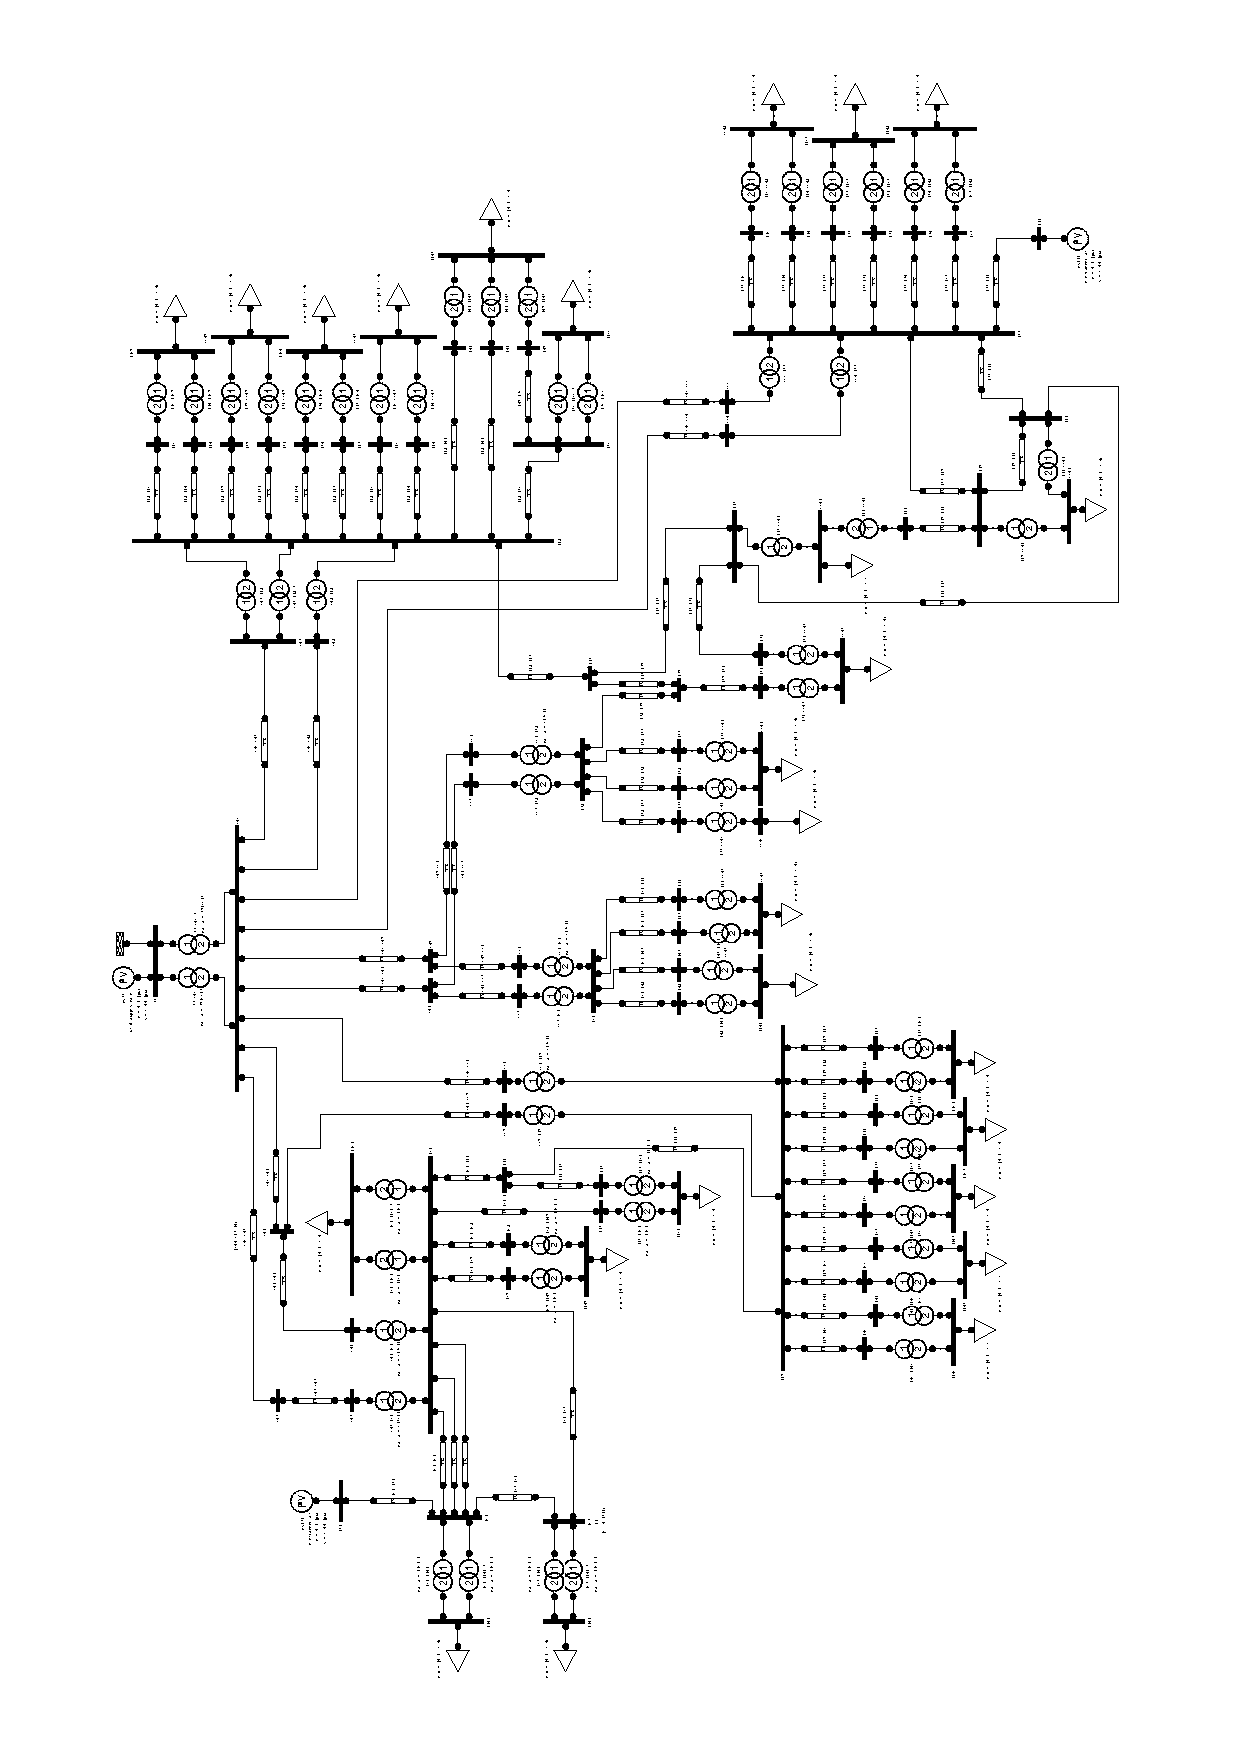
\includegraphics[width=20cm,angle=90]{figures/psat}
	  \caption{UKGDS EHV3 model in PSAT Simulink network editor.}
	  \label{fig:ukgds_ehv3}
	\end{figure}
}{}

Optimal power flow problems are solved via an interface to the General Algebraic
Modeling System (GAMS).  GAMS defines optimisation problems using a high-level
modelling language and has a large solver portfolio that includes all of the
major commercial and academic solvers.  The interface can be used for solving single
period optimal power flow problems where the objective function can model
maximisation of social benefit, maximisation of the distance to the maximum
loading condition or a multi-objective combination of these. Multi-period
optimal power flow is formulated as a mixed integer problem with linearised
power balance constraints.  The objective function models maximisation of social
welfare, but is extended to include start-up and shutdown costs.

Power flow and dynamic data are often separated in electric power
simulation tools, but in PSAT they are integrated.  This combined with the
large number of routines supported by PSAT can make the code base difficult to
understand and modify.  However, comprehensive documentation is included with
PSAT and the mailing list is very active.
%The majority of correspondance on
%this list concerns PSAT's dynamic simulation features.
The price of GAMS
licenses and the need for optimal power flow problems to be converted to the
GAMS language before being solved may be considered barriers to its
selection for certain projects.

\section{UWPFLOW}
% Continuation and Direct Methods to Locate Fold Bifurcations in AC/DC/FACTS
% Power Systems
UWPFLOW is a research tool for voltage stability analysis developed at the
University of Waterloo, Ontario, and the University of Wisconsin-Madison.  It
is written in ANSI-C and is available as open source for research purposes
only. The program can be run with the terminal command
\begin{center}
\begin{verbatim}
$ uwpflow [-options] input_file
\end{verbatim}
\end{center}
where \texttt{input\_file} is the path to a data file in the IEEE common data
format (CDF) \cite{cdf:73}, that may contain High-Voltage Direct Current (HVDC)
and Flexible Alternating Current Transmission System (FACTS) device data.
Output is also in the CDF and can include additional data for post-processing,
including values for nose curve plots.  An interface to UWPFLOW is provided
with PSAT and can be used for bifurcation analysis.

\section{TEFTS}
% Transient Stability Program to Study Energy Functions and Voltage Stability
% (Bifurcation) Phenomena in AC/DC Power Systems
The University of Waterloo also hosts TEFTS -- a transient stability program
for studying energy functions and voltage stability phenomena in AC/HVDC
dynamic power system models.  It too is written in ANSI-C and is licensed for
research purposes only.  An executable file for DOS is provided and the source
package contains a simple example.

\section{VST}
The Voltage Stability Toolbox (VST) is a \matlab toolbox, developed at the
Center for Electric Power Engineering at Drexel University in Philidelphia, for
investigating stability and bifurcation issues in power systems.  The source
is available for any purpose providing that the authors are suitably cited.
VST features routines for:
\begin{itemize}
  \item Power flow,
  \item Time domain simulation,
  \item Static and dynamic bifurcation analysis,
  \item Singularity analysis and
  \item Eigenvalue analysis.
\end{itemize}
The feature matrix in Table \ref{tbl:featurematrix} shows the similar
capabilities of VST and PSAT. It was developed around the same time and has
the same goals for educational and research applications.  However, VST does
not have the same quality of documentation, graphical user interface or such an
active community of users and developers.

\section{OpenDSS}
In November 2008, the Open Distribution System Simulator (OpenDSS) was released
by the Electric Power Research Institute (EPRI) as open source.  Development of
OpenDSS began in April 1997 and it has been used extensively in studies of
distribution systems including distributed generation impact assessments.
% It is the only open source
% program designed for both distribution and transmission system simulation.

OpenDSS supports steady-state analysis in the frequency domain, including power
flow, harmonics and dynamics.  Arbitrary $n$-phase unbalanced circuit analysis
is supported using an object orientated data model.  Circuit elements are
defined in Object Pascal and solutions are obtained using KLUSolve: a linear
sparse matrix solver written in C and \CC and developed specifically for solving
electrical circuits. The OpenDSS Pascal code is available under the Berkeley
Software Distribution (BSD) license, which allows use for almost any purpose.
KLUSolve, is available under the \textsc{Gnu} Lesser GPL. Circuits are defined
in scripts, using a domain specific language, that may be executed through a
graphical user interface or a Common Object Model (COM) interface. The user
interface also provides circuit data editing, plotting and power flow
visualisation tools.

The power flow solver is fast and can be configured for repeated studies using
daily, yearly or duty-cycle data.  The multi-phase circuit model allows complex
transformer models and fault conditions to be defined and three short-circuit
analysis methods are provided.  The heritage of OpenDSS is in harmonics and
dynamics analysis and it does not support system optimisation.

\section{GridLAB-D}
GridLAB-D is an energy system simulation and analysis tool
designed to investigate the latest energy technologies.  The project was
initiated by the U.S.~Department of Energy in 2004 and developed at Pacific
Northwest National Laboratory.  It was released under a BSD-style license in
September 2009 and has since been developed in collaboration with industry and
acedemia.

A distributed simulation architecture is used to coordinate energy system
component interactions over short and long timescales.  The core of GridLAB-D is
made up of modules for simulating: distribution and transmission systems,
commercial and residential buildings, energy markets, power system faults and
meteorological systems.  GridLAB-D is written in \CC~and uses a domain specific
language to define models.  Additional modules can be written in \CC~or Java and
Python is under consideration.  It is designed for multicore/multiprocessor
parallelism and the developers intend to use it simulate large areas of the U.S.
on supercomputers.  The source code includes reports and data from the Olympic
Peninsula Project: a futuristic energy pricing experiment that provides a
practical demonstration of GridLAB-D in operation.

GridLAB-D is a unique simulation tool that has the potential to play an
important role in future energy system development.  Its size and complexity
can make for a steep learning curve, but extensive documentation is provided
and training courses are run periodically.  Activity on the mailing lists is low,
suggesting poor uptake, but the software is actively supported and a new
version is under development.

\section{AMES}
\label{sec:ames}
The AMES (Agent-based Modeling of Electricity Systems) power market testbed is
a software package that models core features of the Wholesale Power Market
Platform: a market design proposed by the Federal Energy Regulatory
Commission (FERC) in April 2003 for common adoption in regions of the
U.S.~\cite{tesfatsi:wpmp}. The market design features:
\begin{itemize}
  \item A centralised structure managed by an independent market operator,
  \item Parallel day-ahead and real-time markets and
  \item Locational marginal pricing.
\end{itemize}
Learning agents represent load serving entities or generating companies and
learn using Roth-Erev reinforcement learning methods,
implemented using the Repast agent simulation toolkit \cite{gieseler:thesis}.
% The permissive license under which the source code for
% these algorithms has been released allowed direct translation of them for use
% in this study.
Agents learn from the solutions of hourly bid/offer based
DC-OPF problems formulated as quadratic programs using the DCOPFJ package
\cite{tesfatsi:dcopf} (See Section \ref{sec:dcopfj}, below).

The capabilities of AMES are demonstrated using a 5-bus network model in
\citeA{tesfatsi:pes09}.  The model is provided with AMES and a step-by-step
tutorial describes how it may be used.  AMES comes with a
Swing-based graphical user interface with plotting and table editor tools and
is released under the \textsc{Gnu} GPL, version 2.

\section{DCOPFJ}
\label{sec:dcopfj}
To solve market problems defined in AMES, researchers at Iowa State University
developed a stand-alone DC optimal power flow solver in Java named DCOPFJ.
It formulates optimal power flow problems as convex quadratic programs
which are solved using QuadProgJ.  The same researcher developed QuadProgJ as
an independent solver that uses a dual active set strictly convex quadratic
programming algorithm \cite{goldfarb:scqp}.  DCOPFJ requires
generator costs to be modelled as polynomial functions, of second order or
less, and does not explot sparse matrix features.

\section{PYLON}
\label{sec:pylon}
% Table \ref{tbl:featurematrix} shows that there are open source software tools
% for all of the main Electric Power Engineering problems and that Matlab is the
% most popular language used.  Several of the projects are more than a decade
% old and the relatively recent release of OpenDSS by EPRI shows that interest
% in this approach to development is not fading.

\pylon is a translation of \matpower v4.0b2 and \textsc{Matdyn} v1.2 to the
Python programming language.  It has extensions for agent-based electricity
market simulation that provide features similar to those of AMES.  Both the DC
and AC formulations of the extensible optimal power flow model from \matpower
are implemented \cite{zimmerman:mp_pes}.  Either a Python version of MIPS or an
interface to IPOPT from COIN-OR can be used to compute solutions.  The sparsity
of the problems is exploited throughout the solution process using matrix
packages from SciPy and bindings to SuperLU or UMFPACK for LU decomposition and
solving sparse sets of linear equations. Scripts are provided for reading and
writing data files in PSS/E, \matpower and PSAT format. A wide variety of
learning methods are available in \pylon due to its use of the PyBrain machine
learning library \cite{schaul:2010}.  PyBrain also provides the artificial
neural network models used for policy function approximation, that may be
accelerated using C extension modules from the ARAC sub-project.

In addition to its market simulation capabilities, \pylon also features solvers
for power flow problems (using fast decoupled or Newton's method), state
estimation, continuation power flow and time domain simulation.  \pylon includes
both a text interface and a graphical user interface (GUI) based on Tkinter:
which is included with Python and imposes no additional dependencies.  A feature
rich GUI is provided by plug-ins for Puddle: an extensible, GUI toolkit
independent integrated development environment, developed for the purposes of
this thesis also.

The use of matrix
libraries from NumPy and SciPy has allowed \pylon (with the permission of the
\matpower developers) to be released under the Apache license, version 2.0. This
allows \pylon to be used as a library in proprietary software as well as
free and open source tools since derivatives of the source code may be made
available under more restrictive terms than the original Apache license.  This
is in contrast to strong ``copyleft'' licenses, such as the \textsc{Gnu} GPL,
that require the same rights to be preserved in modified versions of the work.

\section{Summary}
A diverse range of open source Electric Power Engineering tools are available.
Implementations of most of the traditional power system analysis routines can be
found and many offer performance comparable with proprietary offerings.  Various
programming languages are used, but Matlab is the most popular choice.

Several projects are licensed under the \textsc{Gnu} GPL and it ensures that all
users have access to the full source code.  This does impose restrictions on the
redistribution of projects that use the routines and this can be a barrier to
use in certain types of project.  To encourage commercial use and promote
industrial involvement, two large code bases (OpenDSS and GridLAB-D) have
recently been released under weak copyleft licenses.  Pylon was developed using
specific scientific computing libraries and permission was obtained from the
developers of \matpower to allow release under a similarly permissive license.
Most of the projects described above are led and developed by one individual
and contributions from the user community are typically minimal.  It is hoped
that Pylon's use of a popular free programming language and its liberal
licensing conditions will encourage community involvement and lead to inventive
combinations of simulation routines and web technologies in the
development of intelligent electric power grids.

\chapter{Case Data}
This appendix provides data for the electric power system models used in
Chapters \ref{ch:nashanalysis} and \ref{ch:exploitation}.

\section{6-Bus Case}
\label{adx:case6ww}
The data for the six bus case adapted from \citeA[pp.~104, 112, 119, 123-124,
549]{wood:pgoc} is presented in this section.  The data was imported from the
``case6ww.m'' case file provided with \textsc{Matpower}.
% Figure \ref{fig:case6ww2} illustrates the structure of the model and shows the
% bus injections for the AC unit de-commitment optimal power flow solution.
Table \ref{tbl:case6ww_bus} lists the bus data, Table \ref{tbl:case6ww_gen}
lists the generator data and Table \ref{tbl:case6ww_branch} lists the branch
data.

%\ifthenelse{\boolean{includefigures}}{\begin{figure}
\centering
\begin{scriptsize}
\begin{tikzpicture}[thick]

\tikzstyle{busbar} = [rectangle,draw,fill=black,inner sep=0pt];
\tikzstyle{hbus} = [busbar,minimum width=10mm,minimum height=2pt,drop shadow];

\coordinate (c1) at (0,3);
\coordinate (c2) at (3.5,4.5);
\coordinate (c3) at (7,3);
\coordinate (c4) at (0,0);
\coordinate (c5) at (3.5,-1.5);
\coordinate (c6) at (7,0);
\coordinate (over) at (0,3.75);


\node[hbus,minimum width=20mm,label=left:Bus 1] (b1) at (c1) {};
\node[hbus,minimum width=30mm,label=left:Bus 2] (b2) at (c2) {};
\node[hbus,minimum width=20mm,label=right:Bus 3] (b3) at (c3) {};
\node[hbus,minimum width=20mm,label=left:Bus 4] (b4) at (c4) {};
\node[hbus,minimum width=30mm,label=left:Bus 5] (b5) at (c5) {};
\node[hbus,minimum width=20mm,label=right:Bus 6] (b6) at (c6) {};

% \busbar{b1}{c1}{20mm}
% \busbar{b2}{c2}{40mm}
% \busbar{b3}{c3}{20mm}
% \busbar{b4}{c4}{20mm}
% \busbar{b5}{c5}{40mm}
% \busbar{b6}{c6}{20mm}

% Branch 1-2.
\draw[line] ([xshift=5mm] b1.north) |- ([xshift=-10mm,yshift=-5mm] b2.south) --
([xshift=-10mm] b2.south);
% Branch 1-4.
\draw[line] ([xshift=-5mm] b1.south) -- ([xshift=-5mm] b4.north);
% Branch 1-5.
\draw[line] ([xshift=5mm] b1.south) -- ([xshift=5mm,yshift=-5mm] b1.south)
-- ([xshift=-5mm,yshift=8mm] b5.north) -- ([xshift=-5mm] b5.north);
% Branch 2-3.
\draw[line] ([xshift=10mm] b2.south) -- ++(0,-0.5) -| ([xshift=-5mm]
b3.north);
% Branch 2-4.
\draw[line] ([xshift=-5mm] b2.south) --
([xshift=-5mm,yshift=-8mm] b2.south) -- ([xshift=5mm,yshift=5mm] b4.north)
-- ([xshift=5mm] b4.north);
% Branch 2-5.
\draw[line] (b2.south) -- (b5.north);
% Branch 2-6.
\draw[line] ([xshift=5mm] b2.south) -- ([xshift=5mm,yshift=-8mm] b2.south)
-- ([xshift=-5mm,yshift=5mm] b6.north) -- ([xshift=-5mm] b6.north);
% Branch 3-5.
\draw[line] ([xshift=-5mm] b3.south) -- ([xshift=-5mm,yshift=-5mm] b3.south)
-- ([xshift=5mm,yshift=8mm] b5.north) -- ([xshift=5mm] b5.north);
% Branch 3-6.
\draw[line] ([xshift=5mm] b3.south) -- ([xshift=5mm] b6.north);
% Branch 4-5.
\draw[line] ([xshift=5mm] b4.south) |- ([xshift=-10mm,yshift=5mm] b5.north) --
([xshift=-10mm] b5.north);
% Branch 5-6.
\draw[line] ([xshift=10mm] b5.north) -- ([xshift=10mm,yshift=5mm] b5.north) -|
([xshift=-5mm] b6.south);

% Generator 1.
\genset{g1}{$(c1)+(-5mm,8mm)$}{label=above:110 MW}
\draw[line] ([xshift=-5mm] b1.north) -- (g1.south);
% Generator 2.
\genset{g2}{$(c2)+(0,8mm)$}{label=above:110 MW}
\draw[line] (b2.north) -- (g2.south);
% Generator 3.
\genset{g3}{$(c3)+(5mm,8mm)$}{label=above:220 MW}
\draw[line] ([xshift=5mm] b3.north) -- (g3.south);

% Load 1.
\draw[loadline] ([xshift=-5mm] b4.south) -- ++(0,-0.8) node[text centered,text
width=10mm,below] {70 MW};
% \loadd{l1}{$(c4)-(5mm,15mm)$}
% \draw[line] (l1.south) -- ([xshift=-5mm] b4.south);
% Load 2.
\draw[loadline] (b5.south) -- ++(0,-0.8) node[text centered,text
width=10mm,below] {70 MW};
% \loadd{l2}{$(c5)-(0mm,15mm)$}
% \draw[line] (l2.south) -- (b5.south);
% Load 3.
\draw[loadline] ([xshift=5mm] b6.south) -- ++(0,-0.8) node[text centered,text
width=10mm,below] {70 MW};
% \loadd{l3}{$(c6)+(5mm,-15mm)$}
% \draw[line] (l3.south) -- ([xshift=5mm] b6.south);

\end{tikzpicture}
\end{scriptsize}
\caption{Single-line diagram for six bus power system model.}
\label{fig:case6ww}
\end{figure}
}{}
%\ifthenelse{\boolean{includefigures}}{\input{tikz/case6ww2}}{}

\begin{table}[h]
\caption{6-bus case bus data.}
\label{tbl:case6ww_bus}
\begin{center}
\begin{tabular}{c|c|c|c|c|c|c|c}
\hline
Bus &$P_d$ &$Q_d$ &$G_s$ &$B_s$ &$V_{base}$ &$V_{max}$ &$V_{min}$\\
\hline\hline
%%%%%%%%%%%%%%%%%%%%%%%%%%%%%%%%%%%%%%%%%%%%%%%%%%%%%%%%%%%%%%%%%%%%%%
%%                                                                  %%
%%  This is a LaTeX2e table fragment exported from Gnumeric.        %%
%%                                                                  %%
%%%%%%%%%%%%%%%%%%%%%%%%%%%%%%%%%%%%%%%%%%%%%%%%%%%%%%%%%%%%%%%%%%%%%%
1	&0	&0	&0	&0	&230	&1.05	&1.05\\
2	&0	&0	&0	&0	&230	&1.05	&1.05\\
3	&0	&0	&0	&0	&230	&1.07	&1.07\\
4	&70	&70	&0	&0	&230	&1.05	&0.95\\
5	&70	&70	&0	&0	&230	&1.05	&0.95\\
6	&70	&70	&0	&0	&230	&1.05	&0.95\\

\hline
\end{tabular}
\end{center}
\end{table}

\begin{table}[h]
\caption{6-bus case generator data.}
\label{tbl:case6ww_gen}
\begin{center}
\begin{tabular}{c|c|c|c|c|c}
\hline
Bus &$P_{max}$ &$P_{min}$ &$V_g$ &$Q_{max}$ &$Q_{min}$\\
\hline\hline
%%%%%%%%%%%%%%%%%%%%%%%%%%%%%%%%%%%%%%%%%%%%%%%%%%%%%%%%%%%%%%%%%%%%%%
%%                                                                  %%
%%  This is a LaTeX2e table fragment exported from Gnumeric.        %%
%%                                                                  %%
%%%%%%%%%%%%%%%%%%%%%%%%%%%%%%%%%%%%%%%%%%%%%%%%%%%%%%%%%%%%%%%%%%%%%%
1	&1.05	&200	&50	&100	&-100\\
2	&1.05	&150	&37.5	&100	&-100\\
3	&1.07	&180	&45	&100	&-100\\

\hline
\end{tabular}
\end{center}
\end{table}

\begin{table}[h]
\caption{6-bus case branch data.}
\label{tbl:case6ww_branch}
\begin{center}
\begin{tabular}{c|c|c|c|c|c|c|c}
\hline
From &To &$r$ &$x$ &$b_c$ &$S_{max}$ &$\tau$ &$\theta_{ph}$\\
\hline\hline
%%%%%%%%%%%%%%%%%%%%%%%%%%%%%%%%%%%%%%%%%%%%%%%%%%%%%%%%%%%%%%%%%%%%%%
%%                                                                  %%
%%  This is a LaTeX2e table fragment exported from Gnumeric.        %%
%%                                                                  %%
%%%%%%%%%%%%%%%%%%%%%%%%%%%%%%%%%%%%%%%%%%%%%%%%%%%%%%%%%%%%%%%%%%%%%%
1	&2	&0.1	&0.2	&0.04	&40	&0	&0\\
1	&4	&0.05	&0.2	&0.04	&60	&0	&0\\
1	&5	&0.08	&0.3	&0.06	&40	&0	&0\\
2	&3	&0.05	&0.25	&0.06	&40	&0	&0\\
2	&4	&0.05	&0.1	&0.02	&60	&0	&0\\
2	&5	&0.1	&0.3	&0.04	&30	&0	&0\\
2	&6	&0.07	&0.2	&0.05	&90	&0	&0\\
3	&5	&0.12	&0.26	&0.05	&70	&0	&0\\
3	&6	&0.02	&0.1	&0.02	&80	&0	&0\\
4	&5	&0.2	&0.4	&0.08	&20	&0	&0\\
5	&6	&0.1	&0.3	&0.06	&40	&0	&0\\

\hline
\end{tabular}
\end{center}
\end{table}

\section{IEEE Reliability Test System}
\label{adx:ieee_rts}
This section provides data for the modified IEEE Reliability Test System that
was imported from the ``case24\_ieee\_rts.m'' case file, provided with \matpower
and was originally contributed by Bruce Wollenberg.
Table \ref{tbl:rtsbus} lists the bus data, Table \ref{tbl:rtsgen} lists the
generator data, Table \ref{tbl:rtsbranch} lists the branch data and Table
\ref{tbl:rtsgencost} lists the generator cost data provided by Georgia Tech
Power Systems Control and Automation Laboratory.

%\ifthenelse{\boolean{includefigures}}{\newcommand{\genunit}[3]{
  \node[circle,draw,thick,minimum width=6mm,#3] (#1) at (#2) {};
  \draw[thick] ($(#2)-(2mm,0)$) sin ++(1mm,1mm) cos ++(1mm,-1mm)
  sin ++(1mm,-1mm) cos ++(1mm,1mm);
}

\begin{figure}
\centering
\small
\begin{tikzpicture}[thick,label distance=0mm]
  \tikzstyle{busbar} = [rectangle,draw,fill=black!50,inner sep=0pt];
  \tikzstyle{hbus} = [busbar,minimum width=10mm,minimum height=2pt];
  \tikzstyle{vbus} = [busbar,minimum width=2pt,minimum height=10mm];
  \tikzstyle{overhead} = [-,thick];
  \tikzstyle{cable} = [thick];
  \tikzstyle{trxcircle} = [circle,draw=black,inner sep=0pt,minimum width=5mm];
  \tikzstyle{every pin edge}=[-,shorten <=1pt,thin];

\node[hbus,minimum width=15mm,label=left:Bus 1] (bus1) at (5,0) {};
\node[hbus,minimum width=15mm,label=right:Bus 2] (bus2) at (7,0) {};
\node[hbus,label=right:Bus 3] (bus3) at (0,6) {};
\node[vbus,label=above:Bus 4] (bus4) at (3,4) {};
\node[vbus,label=above:Bus 5] (bus5) at (6.5,3) {};
\node[vbus,label=above:Bus 6] (bus6) at (12,5.3) {};
\node[hbus,label=right:Bus 7] (bus7) at (11,0.5) {};
\node[vbus,label=above:Bus 8] (bus8) at (12,3) {};
\node[hbus,minimum width=20mm,label=left:Bus 9] (bus9) at (5,6) {};
\node[hbus,minimum width=20mm,label=right:Bus 10] (bus10) at (8,6) {};
\node[hbus,minimum width=20mm,label=left:Bus 11] (bus11) at (5,8) {};
\node[hbus,minimum width=20mm,label=right:Bus 12] (bus12) at (8,8) {};
\node[vbus,label={[xshift=-4mm]below:Bus 13}] (bus13) at (12,10) {};
\node[vbus,label=above:Bus 14] (bus14) at (3.5,11.5) {};
\node[hbus,minimum width=20mm,label=right:Bus 15] (bus15) at (0.5,12) {};
\node[hbus,minimum width=15mm,label=right:Bus 16] (bus16) at (0,14) {};
\node[vbus,minimum height=20mm,label=above:Bus 17] (bus17) at (-1,16) {};
\node[hbus,minimum width=20mm,label=right:Bus 18] (bus18) at (2,18) {};
\node[hbus,label=below right:Bus 19] (bus19) at (4.5,14) {};
\node[hbus,minimum width=15mm,label=below right:Bus 20] (bus20) at (7,14) {};
\node[hbus,minimum width=25mm,label=right:Bus 21] (bus21) at (5,17) {};
\node[hbus,label=right:Bus 22] (bus22) at (9,17) {};
\node[vbus,minimum height=15mm,label=above:Bus 23] (bus23) at (11,14.55) {};
\node[hbus,label=right:Bus 24] (bus24) at (0,8) {};

% Branch 1-2.
\draw[cable] ([xshift=5mm] bus1.north) -- ++(0,5mm) node[xshift=5mm,above]
{cable} -| ([xshift=-5mm] bus2.north);
% Branch 1-3.
\draw[overhead] ([xshift=-5mm] bus1.north) -- ([xshift=-5mm,yshift=5mm]
bus1.north) -- ([xshift=0mm,yshift=-5mm] bus3.south) -- (bus3.south);
% Branch 1-5.
\draw[overhead] (bus1.north) |- (bus5.west);
% Branch 2-4.
\draw[overhead] (bus2.north) -- ([yshift=5mm] bus2.north) -- ([xshift=5mm]
bus4.east) -- (bus4.east);
% Branch 2-6.
\draw[overhead] ([xshift=5mm] bus2.north) -- ([xshift=5mm,yshift=5mm]
bus2.north) -- ([xshift=-5mm,yshift=-3mm] bus6.west) -- ([yshift=-3mm]
bus6.west);
% Branche 3-9.
\draw[overhead] ([xshift=3mm] bus3.south) -- ++(0,-5mm) -| ([xshift=-5mm]
bus9.south);
% Branch 3-24.
\draw node[trxcircle,yshift=-1mm,above of=bus3] (t3-24p) {};
\draw node[trxcircle,yshift=1mm,above of=bus3] (t3-24s) {};
\draw[overhead] (bus3.north) -- (t3-24p.south);
\draw[overhead] (t3-24s.north) -- (bus24.south);
% Branch 4-9.
\draw[overhead] ([yshift=3mm] bus4.east) -- ([xshift=5mm,yshift=3mm] bus4.east)
-- ([yshift=-5mm] bus9.south) -- (bus9.south);
% Branch 5-10.
\draw[overhead] (bus5.east) -| (bus10.south);
% Branch 6-10.
\draw[overhead] (bus6.west) -| node[above right] {cable} ([xshift=5mm]
bus10.south);
% Branch 7-8.
\draw[overhead] ([xshift=-3mm] bus7.north) |- ([yshift=-3mm] bus8.west);
% Branch 8-9.
\draw[overhead] (bus8.west) -- ([xshift=-5mm] bus8.west) --
([xshift=5mm,yshift=-5mm] bus9.south) -- ([xshift=5mm] bus9.south);
% Branch 8-10;
\draw[overhead] ([yshift=3mm] bus8.west) -- ([xshift=-5mm,yshift=3mm]
bus8.west) -- ([xshift=-5mm,yshift=-10mm] bus10.south) -- ([xshift=-5mm]
bus10.south);
% Branch 9-11.
\draw node[trxcircle,yshift=-1mm,xshift=-5mm,above of=bus9] (t9-11p) {};
\draw node[trxcircle,yshift=1mm,xshift=-5mm,above of=bus9] (t9-11s) {};
\draw[overhead] ([xshift=-5mm] bus9.north) -- (t9-11p.south);
\draw[overhead] (t9-11s.north) -- ([xshift=-5mm] bus11.south);
% Branch 9-12.
\draw node[trxcircle,yshift=-1mm,xshift=-5mm,node distance=7mm,below of=bus12]
(t9-12p) {};
\draw node[trxcircle,yshift=1mm,xshift=-5mm,node distance=7mm,below of=bus12]
(t9-12s) {};
\draw[overhead] ([xshift=5mm] bus9.north) -- ([xshift=5mm,yshift=3mm]
bus9.north) -- ([yshift=-3mm] t9-12p.south) -- (t9-12p.south);
\draw[overhead] (t9-12s.north) -- ([xshift=-5mm] bus12.south);
% Branch 10-11.
\draw node[trxcircle,yshift=-1mm,xshift=5mm,node distance=7mm,below of=bus11]
(t10-11p) {};
\draw node[trxcircle,yshift=1mm,xshift=5mm,node distance=7mm,below of=bus11]
(t10-11s) {};
\draw[overhead] ([xshift=-5mm] bus10.north) -- ([xshift=-5mm,yshift=3mm]
bus10.north) -- ([yshift=-3mm] t10-11p.south) -- (t10-11p.south);
\draw[overhead] (t10-11s.north) -- ([xshift=5mm] bus11.south);
% Branch 10-12.
\draw node[trxcircle,yshift=-1mm,xshift=5mm,above of=bus10] (t10-12p) {};
\draw node[trxcircle,yshift=1mm,xshift=5mm,above of=bus10] (t10-12s) {};
\draw[overhead] ([xshift=5mm] bus10.north) -- (t10-12p.south);
\draw[overhead] (t10-12s.north) -- ([xshift=5mm] bus12.south);
% Branch 11-13.
\draw[overhead] ([xshift=5mm] bus11.north) -- ([xshift=5mm,yshift=5mm]
bus11.north) -- ([xshift=-5mm] bus13.west) -- (bus13.west);
% Branch 11-14.
\draw[overhead] ([xshift=-5mm] bus11.north) |- ([yshift=-3mm] bus14.east);
% Branch 12-13.
\draw[overhead] ([xshift=-5mm] bus12.north) -- ([xshift=-5mm,yshift=7mm]
bus12.north) -- ([xshift=-5mm,yshift=-3mm] bus13.west) -- ([yshift=-3mm]
bus13.west);
% Branch 12-23.
\draw[overhead] ([xshift=5mm] bus12.north) |- ([yshift=-5mm] bus23.west);
% Branch 13-23.
\draw[overhead] ([yshift=3mm] bus13.west) -- ([xshift=-5mm,yshift=3mm]
bus13.west) |- ([yshift=-5mm] bus23.east);
% Branch 14-16.
\draw[overhead] ([yshift=3mm] bus14.west) -- ([xshift=-6mm,yshift=3mm]
bus14.west) |- ([xshift=5mm,yshift=-5mm] bus16.south) -- ([xshift=5mm]
bus16.south);
% Branch 15-16.
\draw[overhead] ([xshift=-5mm] bus15.north) -- (bus16.south);
% Branches 15-21.
\draw[overhead] (bus15.north) -- ([yshift=5mm] bus15.north) -- ([yshift=-10mm]
bus21.south) -- (bus21.south);
\draw[overhead] ([xshift=5mm] bus15.north) -- ([xshift=5mm,yshift=5mm]
bus15.north) -- ([xshift=5mm,yshift=-10mm] bus21.south) -- ([xshift=5mm]
bus21.south);
% Branch 15-24.
\draw[overhead] ([xshift=-5mm] bus15.south) -- (bus24.north);
% Branch 16-17.
\draw[overhead] ([xshift=-5mm] bus16.north) |- ([yshift=-5mm] bus17.east);
% Branch16-19.
\draw[overhead] ([xshift=5mm] bus16.north) -- ([xshift=5mm,yshift=5mm]
bus16.north) -| ([xshift=-3mm] bus19.north);
% Branch 17-18.
\draw[overhead] ([yshift=5mm] bus17.east) -| ([xshift=-5mm] bus18.south);
% Branch 17-22.
\draw[overhead] (bus17.east) -- ([xshift=20mm] bus17.east) -- ([xshift=20mm,
yshift=-5mm] bus17.east) -| ([xshift=3mm] bus22.south);
% Branches 18-21.
\draw[overhead] (bus18.south) -- ([yshift=-20mm] bus18.south) -|
([xshift=-5mm] bus21.south);
\draw[overhead] ([xshift=5mm] bus18.south) -- ([xshift=5mm,yshift=-15mm]
bus18.south) -| ([xshift=-10mm] bus21.south);
% Branches 19-20.
\draw[overhead] (bus19.north) -- ([yshift=10mm] bus19.north) -|
([xshift=-1.5mm] bus20.north);
\draw[overhead] ([xshift=3mm] bus19.north) -- ([xshift=3mm,yshift=5mm]
bus19.north) -| ([xshift=-4.5mm] bus20.north);
% Branches 20-23.
\draw[overhead] ([xshift=1.5mm] bus20.north) |- ([yshift=5mm] bus23.west);
\draw[overhead] ([xshift=4.5mm] bus20.north) |- (bus23.west);
% Branch 21-22.
\draw[overhead] ([xshift=10mm] bus21.south) -- ([xshift=10mm,yshift=-7.5mm]
bus21.south) -| ([xshift=-3mm] bus22.south);

% Generator @ Bus 1.
\genunit{gen1}{4.5,-0.8}{label=left:192 MW,pin={[pin distance=12mm,text
centered,text width=10.5mm]165:2$\times$U20 2$\times$U76}};
\draw[overhead] ([xshift=-5mm] bus1.south) -- (gen1.north);
% Generator @ Bus 2.
\genunit{gen2}{7.5,-0.8}{label=right:192 MW,pin={[pin distance=12mm,text
centered,text width=10.5mm]15:2$\times$U20 2$\times$U76}};
\draw[overhead] ([xshift=5mm] bus2.south) -- (gen2.north);
% Generator @ Bus 7.
\genunit{gen3}{11,-0.3}{label=right:300 MW,pin=below:3$\times$U100};
\draw[overhead] (bus7.south) -- (gen3.north);
% Generator @ Bus 13.
\genunit{gen4}{12.3,10.9}{label=above:591 MW,pin={[pin distance=8mm]
left:3$\times$U197}};
\draw[overhead] ([yshift=3mm] bus13.east) -- ([yshift=3mm,xshift=2.5mm]
bus13.east) -- (gen4.south);
% Generator @ Bus 14.
\genunit{gen5}{4.3,11.8}{label={[text justified,text
width=15mm]right:Synch. Cond.}}; \draw[overhead] ([yshift=3mm] bus14.east) --
(gen5.west);
% Generator @ Bus 15.
\genunit{gen6}{0.5,11.2}{label={[text centered,text width=10mm]below:215 MW},
pin={[pin distance=5mm,text centered,text width=15mm]-70:5$\times$U12
1$\times$U155}}; \draw[overhead] (bus15.south) -- (gen6.north);
% Generator @ Bus 16.
\genunit{gen7}{0.0,15}{label=right:155 MW};
\draw[overhead] (bus16.north) -- (gen7.south);
% Generator @ Bus 18.
\genunit{gen8}{1.5,18.8}{label=left:400 MW,pin={[pin distance=6mm]below
left:Nuclear}}; \draw[overhead] ([xshift=-5mm] bus18.north) -- (gen8.south);
% Generator @ Bus 21.
\genunit{gen9}{5,17.8}{label=right:400 MW,pin={above right:Nuclear}};
\draw[overhead] (bus21.north) -- (gen9.south);
% Generator @ Bus 22.
\genunit{gen10}{9,17.8}{label=right:300 MW,pin={above:Hydro, 6$\times$U50}};
\draw[overhead] (bus22.north) -- (gen10.south);
% Generator @ Bus 23.
\genunit{gen11}{11.8,15.05}{label=below:660 MW,pin={[text centered,text
width=15mm]above:2$\times$U155 1$\times$U350}};
\draw[overhead] ([yshift=5.05mm] bus23.east) -- (gen11.west);

% Load @ Bus 1.
\draw[loadline] ([xshift=5mm] bus1.south) -- ++(0,-0.8) node[text centered,text
width=10mm,below] {108 MW};
% Load @ Bus 2.
\draw[loadline] ([xshift=-5mm] bus2.south) -- ++(0,-0.8) node[text
centered,text width=10mm,below] {97 MW};
% Load @ Bus 3.
\draw[loadline] ([xshift=-3mm] bus3.south) -- ++(0,-0.8) node[text
centered,text width=10mm,below] {108 MW};
% Load @ Bus 4.
\draw[loadline] ([yshift=-3mm] bus4.east) -- ++(3mm,0) -- ++(0,-0.8)
node[below] {74 MW};
% Load @ Bus 5.
\draw[loadline] ([yshift=-3mm] bus5.east) -- ++(3mm,0) --
++(0,-0.8) node[below] {71 MW};
% Load @ Bus 6.
\draw[loadline] (bus6.east) -- ++(3mm,0) -- ++(0,-0.8) node[below] {136 MW};
% Load @ Bus 7.
\draw[loadline] ([xshift=3mm] bus7.north) -- ++(0,0.8) node[right] {125 MW};
% Load @ Bus 8.
\draw[loadline] (bus8.east) -- ++(3mm,0) -- ++(0,-0.8) node[left] {171 MW};
% Load @ Bus 9.
\draw[loadline] ([xshift=2.5mm] bus9.south) -- ++(0,-1) node[below] {175 MW};
% Load @ Bus 10.
\draw[loadline] ([xshift=7.5mm] bus10.north) -- ++(0,3mm) -- ++(8mm,0)
node[above right] {195 MW};
% Load @ Bus 13.
\draw[loadline] ([yshift=-3mm] bus13.east) -- ++(2.5mm,0) -- ++(0,-1)
node[below] {265 MW};
% Load @ Bus 14.
\draw[loadline] ([yshift=-3mm] bus14.west) -- ++(-3mm,0) -- ++(0,-0.8)
node[below] {194 MW};
% Load @ Bus 15.
\draw[loadline] ([xshift=7mm] bus15.south) -- ++(0,-0.8) node[right]
{317 MW};
% Load @ Bus 16.
\draw[loadline] ([xshift=-5mm] bus16.south) -- ++(0,-0.8) node[text centered,
text width=10mm,below] {100 MW};
% Load @ Bus 18.
\draw[loadline] ([xshift=5mm] bus18.north) -- ++(0,0.8) node[right] {333 MW};
% Load @ Bus 19.
\draw[loadline] (bus19.south) -- ++(0,-0.8) node[right] {181 MW};
% Load @ Bus 20.
\draw[loadline] (bus20.south) -- ++(0,-0.8) node[below] {128 MW};

% Area voltage labels.
\node[draw] at (1,2) {\normalsize{138 kV}};
\node[draw] at (6.5,10.3) {\normalsize{230 kV}};

\end{tikzpicture}
\caption{IEEE Reliability Test System}
\label{fig:ieee79rts}
\end{figure}}{}
%\ifthenelse{\boolean{includefigures}}{\input{tikz/ieee79rts2}}{}

\begin{table}[h]
\caption{IEEE RTS bus data.}
\label{tbl:rtsbus}
\begin{center}
\begin{tabular}{c|c|c|c|c|c|c|c}
\hline
Bus &$P_d$ &$Q_d$ &$G_s$ &$B_s$ &$V_{base}$ &$V_{max}$ &$V_{min}$\\
\hline\hline
%%%%%%%%%%%%%%%%%%%%%%%%%%%%%%%%%%%%%%%%%%%%%%%%%%%%%%%%%%%%%%%%%%%%%%
%%                                                                  %%
%%  This is a LaTeX2e table fragment exported from Gnumeric.        %%
%%                                                                  %%
%%%%%%%%%%%%%%%%%%%%%%%%%%%%%%%%%%%%%%%%%%%%%%%%%%%%%%%%%%%%%%%%%%%%%%
1	&108	&22	&0	&0	&138	&1.05	&0.95\\
2	&97	&20	&0	&0	&138	&1.05	&0.95\\
3	&180	&37	&0	&0	&138	&1.05	&0.95\\
4	&74	&15	&0	&0	&138	&1.05	&0.95\\
5	&71	&14	&0	&0	&138	&1.05	&0.95\\
6	&136	&28	&0	&-100	&138	&1.05	&0.95\\
7	&125	&25	&0	&0	&138	&1.05	&0.95\\
8	&171	&35	&0	&0	&138	&1.05	&0.95\\
9	&175	&36	&0	&0	&138	&1.05	&0.95\\
10	&195	&40	&0	&0	&138	&1.05	&0.95\\
11	&0	&0	&0	&0	&230	&1.05	&0.95\\
12	&0	&0	&0	&0	&230	&1.05	&0.95\\
13	&265	&54	&0	&0	&230	&1.05	&0.95\\
14	&194	&39	&0	&0	&230	&1.05	&0.95\\
15	&317	&64	&0	&0	&230	&1.05	&0.95\\
16	&100	&20	&0	&0	&230	&1.05	&0.95\\
17	&0	&0	&0	&0	&230	&1.05	&0.95\\
18	&333	&68	&0	&0	&230	&1.05	&0.95\\
19	&181	&37	&0	&0	&230	&1.05	&0.95\\
20	&128	&26	&0	&0	&230	&1.05	&0.95\\
21	&0	&0	&0	&0	&230	&1.05	&0.95\\
22	&0	&0	&0	&0	&230	&1.05	&0.95\\
23	&0	&0	&0	&0	&230	&1.05	&0.95\\
24	&0	&0	&0	&0	&230	&1.05	&0.95\\

\hline
\end{tabular}
\end{center}
\end{table}

\begin{table}[h]
\caption{IEEE RTS generator data.}
\label{tbl:rtsgen}
\begin{center}
\begin{tabular}{c|c|c|c|c|c|c}
\hline
Bus &$P_{max}$ &$P_{min}$ &$V_g$ &$Q_{max}$ &$Q_{min}$ &Type\\
\hline\hline
%%%%%%%%%%%%%%%%%%%%%%%%%%%%%%%%%%%%%%%%%%%%%%%%%%%%%%%%%%%%%%%%%%%%%%
%%                                                                  %%
%%  This is a LaTeX2e table fragment exported from Gnumeric.        %%
%%                                                                  %%
%%%%%%%%%%%%%%%%%%%%%%%%%%%%%%%%%%%%%%%%%%%%%%%%%%%%%%%%%%%%%%%%%%%%%%
1	&20	&16	&1.035	&10	&0	&U20\\
1	&20	&16	&1.035	&10	&0	&U20\\
1	&76	&15.2	&1.035	&30	&-25	&U76\\
1	&76	&15.2	&1.035	&30	&-25	&U76\\
2	&20	&16	&1.035	&10	&0	&U20\\
2	&20	&16	&1.035	&10	&0	&U20\\
2	&76	&15.2	&1.035	&30	&-25	&U76\\
2	&76	&15.2	&1.035	&30	&-25	&U76\\
7	&100	&25	&1.025	&60	&0	&U100\\
7	&100	&25	&1.025	&60	&0	&U100\\
7	&100	&25	&1.025	&60	&0	&U100\\
13	&197	&69	&1.02	&80	&0	&U197\\
13	&197	&69	&1.02	&80	&0	&U197\\
13	&197	&69	&1.02	&80	&0	&U197\\
14	&0	&0	&0.98	&200	&-50	&SynCond\\
15	&12	&2.4	&1.014	&6	&0	&U12\\
15	&12	&2.4	&1.014	&6	&0	&U12\\
15	&12	&2.4	&1.014	&6	&0	&U12\\
15	&12	&2.4	&1.014	&6	&0	&U12\\
15	&12	&2.4	&1.014	&6	&0	&U12\\
15	&155	&54.3	&1.014	&80	&-50	&U155\\
16	&155	&54.3	&1.017	&80	&-50	&U155\\
18	&400	&100	&1.05	&200	&-50	&U400\\
21	&400	&100	&1.05	&200	&-50	&U400\\
22	&50	&10	&1.05	&16	&-10	&U50\\
22	&50	&10	&1.05	&16	&-10	&U50\\
22	&50	&10	&1.05	&16	&-10	&U50\\
22	&50	&10	&1.05	&16	&-10	&U50\\
22	&50	&10	&1.05	&16	&-10	&U50\\
22	&50	&10	&1.05	&16	&-10	&U50\\
23	&155	&54.3	&1.05	&80	&-50	&U155\\
23	&155	&54.3	&1.05	&80	&-50	&U155\\
23	&350	&140	&1.05	&150	&-25	&U350\\

\hline
\end{tabular}
\end{center}
\end{table}

\begin{table}[h]
\caption{IEEE RTS branch data.}
\label{tbl:rtsbranch}
\begin{center}
\begin{tabular}{c|c|c|c|c|c|c|c}
\hline
From &To &$r$ &$x$ &$b_c$ &$S_{max}$ &$\tau$ &$\theta_{ph}$\\
\hline\hline
\input{tables/ieee_rts_branch}
\hline
\end{tabular}
\end{center}
\end{table}

\begin{table}[h]
\caption{IEEE RTS generator cost data.}
\label{tbl:rtsgencost}
\begin{center}
\begin{tabular}{c|c|c|c|c|c}
\hline
Gen &$C_{up}$ &$a$ &$b$ &$c$ &Type\\
\hline\hline
%%%%%%%%%%%%%%%%%%%%%%%%%%%%%%%%%%%%%%%%%%%%%%%%%%%%%%%%%%%%%%%%%%%%%%
%%                                                                  %%
%%  This is a LaTeX2e table fragment exported from Gnumeric.        %%
%%                                                                  %%
%%%%%%%%%%%%%%%%%%%%%%%%%%%%%%%%%%%%%%%%%%%%%%%%%%%%%%%%%%%%%%%%%%%%%%
1	&1500	&0	&130	&400.685	&U20\\
2	&1500	&0	&130	&400.685	&U20\\
3	&1500	&0.01414	&16.0811	&212.308	&U76\\
4	&1500	&0.01414	&16.0811	&212.308	&U76\\
5	&1500	&0	&130	&400.685	&U20\\
6	&1500	&0	&130	&400.685	&U20\\
7	&1500	&0.01414	&16.0811	&212.308	&U76\\
8	&1500	&0.01414	&16.0811	&212.308	&U76\\
9	&1500	&0.05267	&43.6615	&781.521	&U100\\
10	&1500	&0.05267	&43.6615	&781.521	&U100\\
11	&1500	&0.05267	&43.6615	&781.521	&U100\\
12	&1500	&0.00717	&48.5804	&832.758	&U197\\
13	&1500	&0.00717	&48.5804	&832.758	&U197\\
14	&1500	&0.00717	&48.5804	&832.758	&U197\\
15	&1500	&0	&0	&0	&SynCond\\
16	&1500	&0.32841	&56.564	&86.3852	&U12\\
17	&1500	&0.32841	&56.564	&86.3852	&U12\\
18	&1500	&0.32841	&56.564	&86.3852	&U12\\
19	&1500	&0.32841	&56.564	&86.3852	&U12\\
20	&1500	&0.32841	&56.564	&86.3852	&U12\\
21	&1500	&0.00834	&12.3883	&382.239	&U155\\
22	&1500	&0.00834	&12.3883	&382.239	&U155\\
23	&1500	&0.00021	&4.4231	&395.375	&U400\\
24	&1500	&0.00021	&4.4231	&395.375	&U400\\
25	&1500	&0	&0.001	&0.001	&U50\\
26	&1500	&0	&0.001	&0.001	&U50\\
27	&1500	&0	&0.001	&0.001	&U50\\
28	&1500	&0	&0.001	&0.001	&U50\\
29	&1500	&0	&0.001	&0.001	&U50\\
30	&1500	&0	&0.001	&0.001	&U50\\
31	&1500	&0.00834	&12.3883	&382.239	&U155\\
32	&1500	&0.00834	&12.3883	&382.239	&U155\\
33	&1500	&0.00490	&11.8495	&665.109	&U350\\

\hline
\end{tabular}
\end{center}
\end{table}
